\documentclass{standalone}
\usepackage{tikz}
\usetikzlibrary{positioning, fit, backgrounds, shapes, arrows.meta}

\begin{document}
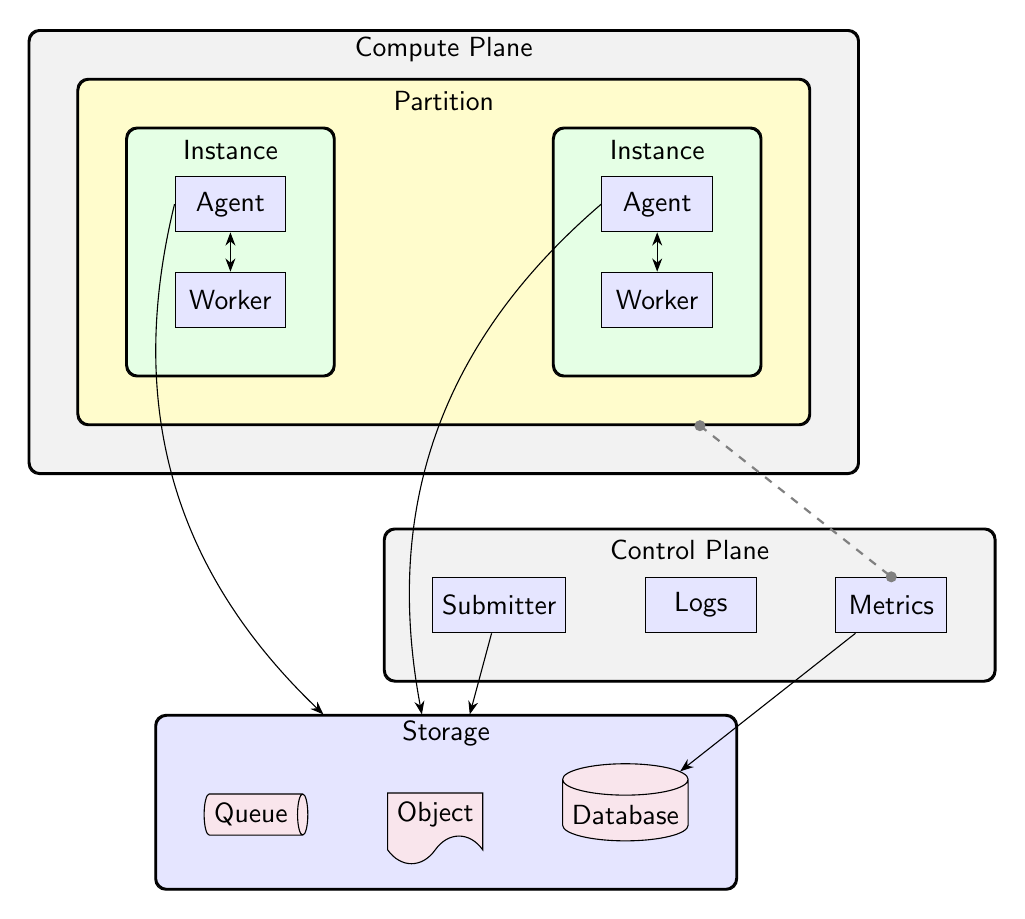
\begin{tikzpicture}[
    font=\sffamily,
    box/.style={
      draw,
      fill=blue!10,
      minimum width=4em,
      minimum height=2em,
      align=center
    },
    object/.style={
      tape,
      tape bend top=none,
      tape bend height=1em,
      fill=purple!10,
      draw,
    },
    database/.style={
      cylinder,
      fill=purple!10,
      aspect=0.25,
      draw,
      shape border rotate=90
    },
    queue/.style={
      cylinder,
      fill=purple!10,
      aspect=0.25,
      draw,
    },
    container/.style={
      draw,
      thick,
      label={[yshift=-3.5ex]north:#1},
      inner sep=4ex,
      rounded corners=4pt
    },
    bg container/.style={
      draw,
      inner sep=0pt,
      fit=#1,
      rounded corners=4pt
  },
  arrow/.style={-Stealth},
  biarrow/.style={Stealth-Stealth},
]

\newcommand{\dashedLineWithDots}[2]{%
  \fill[gray] (#1) circle (2pt);
  \draw[dashed, color=gray, bend right, thick] (#1) -- (#2);
  \fill[gray] (#2) circle (2pt);
}

% Compute Plane
\node[box] (agent1) {Agent};
\node[box, below=0.5cm of agent1] (worker1) {Worker};
\draw[biarrow] (agent1) -- (worker1);

\node[box, right=4cm of agent1] (agent2) {Agent};
\node[box, below=0.5cm of agent2] (worker2) {Worker};
\draw[biarrow] (agent2) -- (worker2);

% Fit Instances
\node[container={Instance}, fit=(agent1)(worker1)] (inst1) {};
\node[container={Instance}, fit=(agent2)(worker2)] (inst2) {};

% Partition
\node[container={Partition}, fit=(inst1)(inst2)] (partition) {};

% Compute Plane
\node[container={Compute Plane}, fit=(partition)] (computeplane) {};

% Control Plane
\node[box, below=1.3cm of computeplane, xshift=2em] (submitter) {Submitter};
\node[box, right=1cm of submitter] (logs) {Logs};
\node[box, right=1cm of logs] (metrics) {Metrics};
\node[container={Control Plane}, fit=(submitter)(metrics)(logs)] (controlplane) {};

% Storage
\node[queue, below left=2cm of controlplane] (queue) {Queue};
\node[object, right=1cm of queue] (object) {Object};
\node[database, right=1cm of object] (database) {Database};
\node[container={Storage}, fit=(queue)(object)(database)] (storage) {};

% Arrows
\draw[arrow, bend right] (agent1.west) to (storage);
\draw[arrow, bend right] (agent2.west) to (storage);
\draw[arrow] (submitter) -- (storage);
\draw[arrow] (metrics) -- (database);

% Dotted line between partition and metrics
\dashedLineWithDots{[xshift=-4em]partition.south east}{metrics.north}

% Fill background of each container
\begin{pgfonlayer}{background}
  \node[bg container={(computeplane)}, fill=gray!10] {};
  \node[bg container={(partition)}, fill=yellow!20] {};
  \node[bg container={(inst1)}, fill=green!10] {};
  \node[bg container={(inst2)}, fill=green!10] {};
  \node[bg container={(controlplane)}, fill=gray!10] {};
  \node[bg container={(storage)}, fill=blue!10] {};
\end{pgfonlayer}

\end{tikzpicture}
\end{document}
